%=================================================================================
%                西南交通大学研究生学位论文LaTeX模板
%=================================================================================

% 使用全局样式swjtuThesis,大部分的模板格式均在样式文件中定义完成
% 单面打印: oneside, 双面打印: twoside
\documentclass[twoside,openany]{swjtuThesis}

% 超链接颜色设置(调试时候使用,方便区分文本和超链接)
%\hypersetup{colorlinks,linkcolor=red,citecolor=green,urlcolor=magenta}
\hypersetup{colorlinks=true,pdfborder={0 0 0},citecolor=black,linkcolor=black,urlcolor=black} % 正式版

% 加载信息
%---------------------------------------------------------------------------------
%                西南交通大学研究生学位论文基本信息
%---------------------------------------------------------------------------------

% 请注意:本文件需用户填写论文的相应信息。

% 论文信息
% 定义申请学位
% 请注意:博士学位候选人输入 Doctor,硕士学位候选人输入 Master
\def\degree{Doctor} 

% 论文中文标题
% 请注意:标题控制在36个汉字以内),其中用 \\ 实现标题换行,单行不得超过18个汉字。
% 		  \underline命令用于实现标题的下划线,请把标题输入在\underline命令的的{}中
%		  V2.0, \underline{}已不再使用。
\cTitle{swjtuThesis V3.0}

% 论文英文标题(72个字符以内,包含空格)
\eTitle{swjtuThesis V3.0}


% 国内图书分类号
%\CI{CLS no.}
\CI{TP181, TP311}
% 国际图书分类号
%\UDC{UNC no.}
\UDC{004.8}
% 保密等级
\secLevel{公开}
% 单位代码
\UCODE{10613}

%----------------------------
% 学生信息
% 中英文姓名
\cAuthor{\#\quad \#} % 盲审使用 \author{\#\#\#}
\eAuthor{\#\#\#} % 盲审使用 \eAuthor{\#\#\#}

% 专业(10个汉字以内)
% 请注意:对于超过10个汉字的专业,比如“防灾减灾工程及防护工程”,目前排版仍然不够美观,正在修正。
%        也请相应专业的同学提供过往师兄的硕士论文以供参考。
\cDiscipline{计算机科学与技术}
\eDisciplineFirst{Computer Science and} % 第一行
\eDisciplineSecond{Technology} % 第二行,可为空

% 学号
\studentID{1111223333}

% 导师(10个汉字以内)
% 请注意:导师姓名和导师的职称之间加上\hspace{0.1em}以增大间距,整体显得更为美观。 
%\cTutor{导师\hspace{0.1em} 教授/博导}
%\eTutor{Professor Supervisor Name}
\cTutor{***} % \cTutor{***\hspace{0.1em} 教授}, 盲审使用-> \cTutor{***}
\eTutor{***} % \eTutor{Professor ***}, 盲审使用-> \eTutor{***}

% 学院
\cSchool{计算机与人工智能学院}
\eSchoolFirst{School of Computing and} % 第一行
\eSchoolSecond{Artificial Intelligence} % 第二行,可为空

% 封面日期,依次为年,月,日
\cDate{2024}{7}{4}
\eDate{2024}{Jul.}{4} % 例如,{2024}{May}				% 加载论文信息
%---------------------------------------------------------------------------------
%                判断学位论文类型(硕士学位or博士学位)
%---------------------------------------------------------------------------------

% 请注意:本文件已经定义好需要使用的字符串,不建议用户更改。

\newif\ifdegreedoctor
\newif\ifdegreemaster

\def\temp{Doctor}
\ifx\temp\degree
\degreedoctortrue  \degreemasterfalse
\fi

\def\temp{Master}
\ifx\temp\degree
\degreedoctorfalse  \degreemastertrue
\fi

\ifdegreedoctor
\newcommand{\fitDegree}{博\quad 士}
\newcommand{\cDegree}{博士}
\newcommand{\eDegree}{Doctor of }
\fi

\ifdegreemaster
\newcommand{\fitDegree}{硕\quad 士}
\newcommand{\cDegree}{硕士}
\newcommand{\eDegree}{Master of }
\fi    			% 区分硕博类型(模板自动区分,在info.tex中进行设置)
%---------------------------------------------------------------------------------
%                学位论文LaTeX模板使用宏包文件
%---------------------------------------------------------------------------------

% 数学公式常用宏包(实现更多样的数学公式输入)
\usepackage{amsmath}
\usepackage{amssymb} % AMSLaTeX宏包, 用来排出更加漂亮的公式, 可以使用\eqref{*}而非(ref{*})来引用公式
\usepackage{mathrsfs} % 不同于\mathcal or \mathfrak 之类的英文花体字体
\usepackage{mathtools}
\usepackage{wasysym}
\usepackage{cases} % cases环境
%\usepackage{theorem}
\usepackage[amsmath,thmmarks]{ntheorem} % 定理类环境宏包,其中 amsmath 选项, 用来兼容 AMS LaTeX 的宏包. 与theorem不能同时使用.

% 算法宏包
\usepackage{algorithmic}
\usepackage[lined,boxed,ruled,algochapter]{algorithm2e} % algochapter算法按章编号
\renewcommand{\algorithmcfname}{算法}

% 额外的图表排列控制
\usepackage{float}

% 表格制作常用宏包
\usepackage{multirow}

% 插入图片常用宏包(实现多种格式的调用)
\usepackage{graphicx}
\usepackage{subfig}

% 图表题注格式宏包(实现《规范》要求的题注格式)
% V3.0更改——参考兰大等学校的已发表毕业论文格式,多行图表题的行距变更为1.2倍
\usepackage{caption}
\captionsetup{labelformat=simple, labelsep=quad, labelfont=bf, textfont=normalfont, font={stretch=1.2}}

% TeX系列标识的正确输入宏包(实现正确插入TeX相关的字符串)
\usepackage{dtk-logos}

% 列表制作常用宏包(用于调用小间距列表)
\usepackage{paralist}

% 外框宏包
\usepackage{framed}

% 引用文献宏包natbib
%               上标	方括号	逗号分隔	自动排序分类
\RequirePackage[super,square,comma,sort&compress]{natbib}

% 颜色控制宏包
\usepackage{color,xcolor}
\usepackage{colortbl} %控制表格颜色

% 列表宏包
% V3.0更改——参考已发表论文格式,调整列表元素的缩进选项,达到首行缩进2字符的效果,同时去除了列表与正文的额外间隔
\usepackage{enumerate} % 其后可接选项[a,A,i,I,1]
\usepackage{enumitem}
\setenumerate[1]{itemsep=0pt,partopsep=0pt,parsep=\parskip,topsep=0pt,leftmargin=0pt,itemindent=3.5em}
\setitemize[1]{itemsep=0pt,partopsep=0pt,parsep=\parskip,topsep=0pt,leftmargin=0pt,itemindent=3.5em}
\setdescription{itemsep=0pt,partopsep=0pt,parsep=\parskip,topsep=0pt,leftmargin=0pt,itemindent=3.5em}

% 英文采用Times New Rome字体(建议把这个宏包放在最后避免发生宏包冲突)
\usepackage{fontspec}
\setmainfont{Times New Roman}
% V3.0更改——Times New Roman下强制使用AMS中的黑板体
\DeclareMathAlphabet{\mathbb}{U}{msb}{m}{n}
% 不需要设置CJKmainfont,ctex 宏包已经很好的处理了
% 不仅设置了粗体为黑体,斜体为楷体,还兼容了winfonts和adobefonts
			% 加载使用宏包

% 调整浮动体与文字间距
\setlength{\textfloatsep}{10pt}
\setlength{\intextsep}{10pt}
\setlength{\floatsep}{10pt}

\begin{document}

%---------------------------------------------------------------------------------
% 封面生成(包括中、英文封面、版权协议以及硕(博)士主要工作简述)
\pdfbookmark[0]{封面}{Cover}
\makecover

% 论文前言(包括中、英文摘要及目录,页码为罗马数字,在研究生论文目录中不显示摘要)
\frontmatter
\pagenumbering{Roman}
\thesispagestyle{\leftmark}{\thepage}	% 页眉设置

% 加载中文摘要
\pdfbookmark[0]{中英文摘要}{Abstract}
%---------------------------------------------------------------------------------
%                西南交通大学研究生学位论文:中文摘要
%---------------------------------------------------------------------------------

% 中文摘要输入区A
\cabstract
{
这里是中文摘要输入区。



}
{关键词1,关键词2,关键词3,关键词4,关键词5}
% 中文关键词输入区,基于2024年新规范,关键词之间使用逗号“,”隔开,3~8个

% 加载英文摘要
%---------------------------------------------------------------------------------
%                西南交通大学研究生学位论文:英文摘要
%---------------------------------------------------------------------------------

% 英文摘要输入区
\eabstract
{
Here is for you to write the English abstract.



}
{keyword1; keyword2; keyword3; keyword4; keyword5}	% 英文关键词输入区,关键词之间用“; ”分开,不超过五个

% 目录生成
\pdfbookmark[0]{目录}{Content}
\tableofcontents

%---------------------------------------------------------------------------------
% 学位论文正文(包含各章节内容和结论,页码为阿拉伯数字)
\mainmatter
\thesispagestyle{西南交通大学硕/博士学位论文}{\thepage}	% 页眉设置

% 加载论文正文(第1章 - 第N章、结论)
% 目前共有四个章节文件,用户可以自行在content/:文件夹中添加chap0X.tex文件
% 若新增文件为content/chap_name.tex, 则在这里直接通过\include{content/chap_name}来包含该章节内容

% V3.0更改——调整允许跨页的强度,0--4,越大则更偏向于跨页显示
\allowdisplaybreaks[4]

% V3.0更改——表格字体默认为五号
\AtBeginEnvironment{tabular}{\tiny}

% 为了防止影响封面设置,正文图表题间距设定与被移动至此
% 新模版中明确规定单倍行距
% \renewcommand\arraystretch{1.5}

%---------------------------------------------------------------------------------
%                西南交通大学研究生学位论文:第一章内容
%---------------------------------------------------------------------------------

\chapter{模板介绍}

\LaTeX{}~作为一种具有标记语言(markup language)特色的排版系统(word processors),不同于Microsoft Office Word\textsuperscript{\textregistered}、Apple Pages\textsuperscript{\textregistered}等目前常用的“所见即所得”(what you see is what you get, WYSIWYG)形式页面排版软件,得益于标记语言的特点,其对数学公式、矢量图表、参考文献、交叉引用、格式统一等有着更为良好的支持和表现效果,常应用于在科学研究领域。诸多科技出版社(如Springer\footnote{更多信息请参阅Springer出版社书籍投稿说明:\url{https://www.springer.com/gp/authors-editors/book-authors-editors/manuscript-preparation/5636}}、Elsevier\footnote{更多信息请参阅Elsevier出版社采用\LaTeX{}投稿科学书籍的指南:\url{https://www.elsevier.com/authors/author-schemas/latex-instructions}}等公开出版的学术书籍),科学期刊杂志(如IEEE Transactions系列汇刊\footnote{IEEE论文投稿页面中提供了涵盖了几乎所有汇刊适用的\LaTeX{}模板资源:\url{https://www.ieee.org/publications_standards/publications/authors/author_templates.html}}),国、内外高等学府的学位论文\footnote{\LaTeX 开源小屋网站上提供了许多高校的模板供下载使用:\url{http://www.latexstudio.net}}均有提供现成~\LaTeX{}~模板供作者使用。

\par
\textbf{swjtuThesis正是为了能够让更多的交大学生接触并了解~\LaTeX{},同时能够更为方便地使用~\LaTeX{}~进行研究生学位论文撰写的西南交通大学研究生学位论文~\LaTeX{}~模板}。本模板严格依照《西南交通大学研究生学位论文撰写规范》\footnote{详细信息请参阅西南交通大学研究生院网站页面:\url{http://gs.swjtu.edu.cn/ws/gs/r/719}}进行开发,但由于个人水平有限,难免存在不足之处,欢迎大家积极反馈在使用过程中遇到的问题,或者是对swjtuThesis模板的开发建议,同时也希望能在众多交大~\LaTeX{}~爱好者的努力下,一同完善本模板,受益更多的交大同学。


\section{模板获取}

\textbf{swjtuThesisV3.0基于swjtuThesisV1.0~\footnote{swjtuThesisV1.0: \url{https://github.com/Studio513/swjtuThesis}}以及swjtuThesisV2.0~\footnote{swjtuThesisV2.0: \url{https://github.com/cshaowang/swjtuThesisV2.0}}进行修订(尤其是页面效果设置、三线表设置、行距设置、Mac系统兼容性设置以及参考文献格式的兼容性优化)}。swjtuThesisV3.0(以下简称swjtuThesis或V3.0)模板的所有源代码和资源均作为开源项目的形式托管于GitHub仓库之中,链接地址如下
\par
\begin{center}
	\url{https://github.com/Sophie10001b/swjtuThesisV3.0}
\end{center}
\par
\textbf{通过GitHub直接下载是目前获取swjtuThesis模板及后续更新的稳定途径之一}。目前的swjtuThesis V3.0模板仍然处于Demo阶段,在作者本人的论文通过最终审查前,本模板的相关设置有极大概率被进一步的更改与优化,直至最后形成正式的V3.0版本。特别说明,本模板尚未取得西南交通大学学校方面的认证。V3.0仍是一个处在开发与更新之中的版本。欢迎大家的反馈意见和更新,以及基于当前版本直接推出优化后的新版本,一起推动~\LaTeX{}~在研究生学位论文写作中的普及。

\section{开发环境}

\LaTeX{}~开发环境可以灵活地在Windows、Mac OS及Linux/Ubuntu等主流操作系统中进行配置,对于初学者而言,推荐采用\textbf{~\TeX~发行版}(distribution)配合\textbf{~\TeX~编辑器}(integrated writing environment)的方式进行撰写和开发。

\par
\textbf{对于~\TeX~发行版的选择},Windows操作系统下推荐使用CTeX中文套装(最新版本:CTeX 2.9.2.164\footnote{CTeX下载地址:\url{http://www.ctex.org/CTeXDownload}})或者TeX Live套装(最新版本:TeX Live 2020\footnote{TeX Live下载地址:\url{https://www.tug.org/texlive/}});Linux系统下同样推荐使用TeX Live套装(最新版本:TeX Live 2020);Mac系统下推荐使用MacTeX(最新版本:MacTeX-2020\footnote{MacTeX下载地址:\url{https://tug.org/mactex/}})。

\par
\textbf{对于~\TeX~编辑器的选择},TeXStudio\footnote{TeXStudio下载地址:\url{http://www.ctex.org/CTeXDownload}}和Texmaker\footnote{Texmaker下载地址:\url{https://www.tug.org/texlive/}}均是Windows端的免费的~\LaTeX{}~开发利器,其代码高亮、代码补全、字典功能均比较完善,此外用户可以选择使用WinEdt\footnote{WinEdt官方网站:\url{http://www.winedt.com/}},这是一款功能强大的~\TeX~商业编辑器软件,不过CTex中内置了这款编辑器;Linux系统下同样推荐使用TeXStudio或者Texmaker;Mac系统下的~\TeX~编辑器选择要更为多样,出了之前推荐的之外还有像Texpad\footnote{Texpad官方网站:\url{https://www.texpadapp.com/osx}}之类Mac系统独占的专业~\TeX~编辑器。

\par
\textbf{swjtuThesis模板所采用的开发环境为}:TeX Live 2020 + TeXStudio + XeLaTeX。

\par
\textbf{swjtuThesis V3.0目前已经额外在macOS中通过编译测试,注意在macOS下需要额外下载缺失的字体文件。macOS下模板所采用的开发环境为}:MacTeX 2023 + VSCode(LaTeX Workshop) + XeLaTeX。

\section{模板构成}

西南交通大学研究生学位论文\textbf{swjtuThesis模板中包含的关键文件说明如下}:

\par
\begin{itemize}
  \item \textbf{main.tex}:主文件,\textbf{撰写完成后编译该文件即可产生学位论文.pdf全文};
  \item \textbf{main.pdf}:即当前.pdf文档,也即是\textbf{最终的论文文档},通过编译main.tex产生;
  \item \textbf{swjtuThesis.cls}:文档类文件,基于ctexbook文档类修改,\textbf{不建议用户修改};
  \item \textbf{swjtuThesis.cfg}:文档类文件的配置文件,用于字符串定义,\textbf{不建议用户修改};
  \item \textbf{swjtuBST.bst}:文献引用输出的格式控制文件,用于定义文献引用的输出样式,\textbf{不建议用户修改};
\end{itemize}

\par
此外,在使用过程中将会产生如.aux、.bbl、.log、.out等后缀的文件,均属于~\LaTeX{}~编译过程的正常文件,请用户不要擅自删除或者修改。

\par
swjtuThesis模板中的文件夹目录信息如表\ref{tab_1_1_files}所示。其中,注明\textbf{无需修改}字样的文件为模板已经写好的文件,非特殊情况下不建议用户进行修改;注明\textbf{用户修改}字样的文件请用户自行根据文件中的注释提示予以录入信息,详细的模板使用方法请见第二部分;注明\textbf{用户撰写}字样的文件为空白文件,需要用户自行根据自己的论文需求进行撰写(包括了各章节的内容、致谢、附录、科研成果等等);对于学位论文中所引用全部的参考文献,推荐用户构建~\BibTeX~文献库,并将.bib库文件放置于ref文件夹中,并在main.tex文件中予以调用,即可在swjtuThesis模板中实现对需要的参考文献进行引用,更多关于如何使用~\BibTeX~管理参考文献的使用实例请见第二部分;最后,本模板虽然已经能够实现根据用户输入的信息自行判断学位论文的\textbf{硕、博士}类型,但是关于\textbf{《博士创新声明》}及\textbf{《硕士主要工作》}文件请用户自行打开相应.tex文件在用户撰写区中进行修改。

\begin{table}[htbp]
	\setlength{\abovecaptionskip}{0pt}
	\setlength{\belowcaptionskip}{0pt}\
	\caption{swjtuThesis模板文件夹构成}
	\label{tab_1_1_files}
	\centering
	\begin{tabular}{llll}
		\toprule
		文件夹 & 文件 & 作用说明 & 使用说明 \\
		\midrule
		\multirow{3}{*}{\centering setup\textbackslash{}:} & info.tex & 录入论文信息 & \textbf{用户修改} \\
		& type.tex & 判定论文种类 & \textbf{无需修改} \\
	    & package.tex & 增加使用宏包 & \textbf{用户修改} \\
	    \midrule
	    \multirow{5}{*}{\centering preface\textbackslash{}:} & copyright.tex & 学位论文版权授权书 & \textbf{无需修改} \\
	    & statementDoctor.tex & 博士学位论文创新声明 & \textbf{博士修改} \\
	    & statementMaster.tex & 硕士学位论文主要工作 & \textbf{硕士修改} \\
	    & cabstract.tex & 中文摘要 & \textbf{用户撰写} \\
	    & eabstract.tex & 英文摘要 & \textbf{用户撰写} \\
	    \midrule
	    \multirow{2}{*}{\centering content\textbackslash{}:} & chapN.tex & 第N章内容 & \textbf{用户撰写} \\
	    & conclusion.tex & 结论 & \textbf{用户撰写} \\
	    \midrule
	    \multirow{3}{*}{\centering appendix\textbackslash{}:} & remerciement.tex & 致谢 & \textbf{用户撰写} \\
	    & appX.tex & 附录 & \textbf{用户撰写} \\
	    & myWork.tex & 科研成果 & \textbf{用户撰写} \\
	    \midrule
	    \multirow{2}{*}{\centering ref\textbackslash{}:} & chinesebst.bst & 参考文献样式文件 & \textbf{无需修改} \\
	    & refEx.bib & 参考文献~\BibTeX~数据库 & \textbf{用户录入}\\
	    \midrule
	    figures\textbackslash{}: &  & 放置论文插图 \\
		\bottomrule
	\end{tabular}
\end{table}





%---------------------------------------------------------------------------------
%                西南交通大学研究生学位论文:第二章内容
%---------------------------------------------------------------------------------
\chapter{模板使用}

本章节主要介绍使用swjtuThesis模板进行研究生学位论文撰写的基本方法,更多的~\LaTeX{}~排版介绍和方式方法请参考本章节最后推荐的参考书目。

\section{信息录入}
swjtuThesis模板的信息录入主要包括\textbf{学位论文基本信息}以及用户排版过程中需要增添的\textbf{~\LaTeX{}~宏包信息}两个方面。

\subsection{论文信息}
论文信息主要涵盖拟申请的学位种类(硕士、博士以及学科类别),研究生个人资料(姓名、年级、专业、导师),论文中、英文标题,国内图书分类号\footnote{国内图书分类号(Classified Index)的查询网址:\url{http://www.ztflh.com/}}、国际图书分类法\footnote{国际图书分类法(U.D.C)的查询网址:\url{http://www.udcc.org/udcsummary/php/index.php}}等,\textbf{上述列举的信息均统一在~setup\textbackslash{}info.tex~文件中予以录入}。更详细的说明请参见~setup\textbackslash{}info.tex~文件中的注释语句,参照注释将引导用户完成论文基本信息的录入。

\par
\textbf{在用户完成学位论文基本信息的录入之后,本模板将自动生成硕士、博士学位论文相对应的基本框架},主要包括论文中、英文封面格式,论文页眉格式,以及自动判定加载《博士学位论文创新说明》或者《硕士学位论文主要工作》,此外还有论文结尾处攻读学位论文中所取得的科研成果,\textbf{以上论文格式均无需用户修改。}

\subsection{增加宏包}
为方便管理,\textbf{所有用户需要使用的宏包建议统一放置于~setup\textbackslash{}package.tex~文件夹中}。\LaTeX{}~排版系统中的宏包相当于C编程语言中的头文件,集成了用户需要的一些额外功能(比如amsmath宏包可以实现更加更多功能的数学公式输入,graphicx宏包能够实现直接插入pdf图像,此外还有列表环境的宏包,表格环境的宏包等等)\footnote{用户安装的CTex或者是TeX Live等~\LaTeX{}~发行版已经内置了许多的宏包,用户只需要直接调用即可,不需要额外下载}。\textbf{正因为~\LaTeX{}~能够支持各种各类的拓展性宏包, 才使得其排版功能更加的强大和完善。}更详细的说明请参见~setup\textbackslash{}package.tex~中的注释语句,初始状态下swjtuThesis已经添加了几个比较常用的宏包。



\section{正文撰写}

\subsection{入门书籍}
使用~\LaTeX{}~进行科学排版的方法并非在此三言两语即可解释清楚,目前已经有许多前辈的教程或者手册可供用户入门及学习,学习的参考实体书在此\textbf{重点推荐电子工业出版社2013年出版的刘海洋老师的《\LaTeX{}入门》}\footnote{《\LaTeX{}入门》的其中一个网购链接:\url{http://product.dangdang.com/23252576.html}},该书内容翔实,无论作为~\LaTeX{}~的启蒙读物或者是作为~\LaTeX{}~排版的手册使用都有一定参考价值。

\par
此外,推荐黄新刚老师的个人笔记《\LaTeX{}~Note》(最后更新于2013 年)\footnote{\LaTeX{}~Note下载地址:\url{http://www.dralpha.com/zh/tech/lnotes2.pdf}},简短简洁地介绍了~\LaTeX{}~的使用方式以及一些常用宏包和工具,可作为~\LaTeX{}~排版的入门基本读物。需要注意的是,熟读这本小册子虽然可以掌握一定的~\LaTeX{}~排版技巧,但是由于是个人笔记体的形式,对于一些深入的使用方法还是需要查阅更多的资料。

\par
最后,再推荐三本Springer出版社关于~\LaTeX{}~的书籍,由于交大购买了Springer出版社2002-2015年出版物的数据库,因此使用交大的网络IP就可以直接进行下载。
\begin{publist}
	\item George Grätzer, \emph{More Math Into Latex}, Springer, 2007\footnote{下载链接:\url{http://link.springer.com/book/10.1007/978-0-387-68852-7}}
	\item M. R. C. van Dongen, \emph{\LaTeX{}~and~Friends}, Springer-Verlag Berlin Heidelberg, 2012\footnote{下载链接:\url{http://link.springer.com/book/10.1007/978-3-642-23816-1}}
	\item George Grätzer, \emph{Practical LaTeX}, Springer, 2014\footnote{下载链接:\url{http://link.springer.com/book/10.1007/978-3-319-06425-3}}
\end{publist}

\textbf{建议用户先掌握必要的~\LaTeX{}~排版知识再使用swjtuThesis进行学位论文的撰写}。接下来主要对\textbf{公式编辑}和\textbf{图表绘制}两部分进行说明,也即是~\LaTeX{}~排版的优势所在。

\subsection{公式编辑}
\textbf{对数学公式输入及排版的良好支持和优异表现是~\LaTeX{}~深受科研人员喜爱的重要原因之一},比如需要在正文中插入\textbf{行内公式}时,对于非矩阵和非多行形式的行内公式,如斯托克斯定理:$\int_S\left( \nabla\times \mathbf{A}\right)  \;\mathrm{d}\mathbf{S}=\oint_C \mathbf{A} \;\mathrm{d}\mathbf{l}$,\LaTeX{}~排版系统能够做到很好地对行距进行控制,而Word等软件却往往会根据行内公式的竖直距离而自动调节行距,从而破坏了学位论文的美观性。

\par
接下来是一个\textbf{行间公式}的例子,也就是带有公式号码可以在文中引用的公式
\begin{equation}\label{ch2:divTheo}
	\int_V \left( \nabla \cdot \mathbf{A} \right)  \;\mathrm{d}v = \oint_S \mathbf{A} \;\mathrm{d}\mathbf{s}
\end{equation}

\par
接下来是一个多行的行间公式例子,其中每一行最后不需要单独带有标号
\begin{eqnarray}\label{ch2:Maxwell}
\nabla \times \mathbf{E} &=& - \frac{\partial \mathbf{B}}{\partial t} \nonumber \\
\nabla \times \mathbf{H} &=& \mathbf{J} + \frac{\partial \mathbf{D}}{\partial t}  \nonumber \\
\nabla \cdot \mathbf{D} &=& \rho_v \nonumber \\
\nabla \cdot \mathbf{B} &=& 0
\end{eqnarray}

\par
式(\ref{ch2:Maxwell})正是电磁场里让多少人神魂颠倒的麦克斯韦方程组。

\par
通常情况下~\LaTeX{}~中的数学公式均通过编写代码的形式实现。比如刚才使用的行内公式斯托克斯定理$\int_S\left( \nabla\times \mathbf{A}\right)  \;\mathrm{d}\mathbf{S}=\oint_C \mathbf{A} \;\mathrm{d}\mathbf{l}$,其~\LaTeX{}~代码如下

\begin{framed}
	\begin{verbatim}
	$\int_S\left( \nabla\times \mathbf{A}\right)  \;\mathrm{d}\mathbf{S}
		=\oint_C \mathbf{A} \;\mathrm{d}\mathbf{l}$
	\end{verbatim}
\end{framed}


由上述的代码片段可以看出,插入行内公式的标志语为两个美元符号,也即是\verb|$...$|。其余公式的输入方式大家可以参考刚才提到的参考书籍,也可以直接查阅本模板的初始代码学习。Word中常用的MathType公式编辑器也可以支持编辑公式之后直接复制导出~\LaTeX{}~代码,具体在MathType的选项菜单中可以设置复制为~\LaTeX{}~格式即可。这样可以实现所见即所得的数学公式~\LaTeX{}~编写。不过相对来说基于代码的编辑要更加底层也更为细致。

\subsection{图表绘制}
\textbf{使用~\LaTeX{}~进行科学排版的另一大优势就是可以灵活地在文章中插入矢量绘图},虽然在Word软件也支持插入同为Microsoft Office套件的Visio编辑的矢量图,然而Word其对其余主流矢量图格式(如.pdf, .eps等文件)的支持并不理想。图\ref{SWJTU_LOGO_PNG}和图\ref{SWJTU_LOGO_PDF}分别示出了位图格式和矢量格式的西南交通大学校徽\footnote{请注意,文中所使用的西南交通大学校徽文件中,位图版为采西南交通大学官方提供的校徽LOGO文件,矢量版校徽为模板作者通过软件自行勾勒得出,非官方的正式版,请不要在正式场合使用。},可以看出在放大比率为200\%的时候,位图校徽的边缘开始出现模糊的情形。与此同时,\textbf{由于矢量图是一种基于纯数学公式语言的绘图,采用矢量图制作的插图能够保证成像不会因为放大而失真同时保证很小的文件大小}。

\par
需要注意的是,并非所有的插图都适合采用矢量格式,尤其是照片之类的图片,通常情况下适宜采用.png或者.jpeg等位图格式;\textbf{而系统框图、曲线图、概念流程图等,则以采用矢量图格式为佳。}

\par
目前,主流的商业矢量插画绘制软件以ADOBE公司的Illustrator以及Corel公司的CorelDRAW为主,不过受制于其售价,一般学生用户可以使用一些免费的矢量图编辑软件,例如Inkscape\footnote{Inkscape官方网站:\url{https://inkscape.org/en/}},作为一款矢量图绘制的利器,其功能已经能够基本满足正常的需,深受广大用户的喜爱。

\begin{figure}[htbp]
	\centering
	
\includegraphics[width=3in]{figures/SWJTU_LOGO.png}
	\caption{西南交通大学校徽位图格式(.png)}
	\label{SWJTU_LOGO_PNG}
\end{figure}

\begin{figure}[htbp]
	\centering
	
\includegraphics[width=3in]{figures/SWJTU_LOGO.pdf}
	\caption{西南交通大学校徽矢量格式(.pdf)}
	\label{SWJTU_LOGO_PDF}
\end{figure}



\section{参考文献}
建立一个强大高效的个人文献管理系统能够使科研工作的进展更为科学系统,目前,主流的文献管理软件有EndNote,NoteExpress及免费的Mendeley及Zotero等等。文献管理软件虽然种类繁多,但本质上并无多大的差异,均能够满足科研工作者的正常需求。然而,\textbf{为更为高效地配合~\LaTeX{}~进行排版,在此推荐采用~\BibTeX{}~作为主要的文献管理系统,同时采用JabRef\footnote{JabRef软件网站:\url{http://jabref.sourceforge.net/}}作为文献管理软件,实现文献的导入和引用}。采用~\BibTeX{}~进行文献管理,其核心思想为通过一定的语句格式对参考文献进行的录入,同时把所有学位论文中需要引用的文献集中到一个.bib的库文件中,然后在swjtuThesis模板中加载文献库文件,实现调用所需要的参考文献。

\par
在JabRef软件正常安装之后,可以直接打开模板中内置的参考文献库示范文件refEx.bib,以了解基本的使用方式。然而,\textbf{建议用户不要直接在refEx.bib库文件中直接进行修改,自行建立学位论文所要引用的参考文献库文件(如refs.bib文件),并放于ref文件夹中,在mian.tex文件中予以调用即可}(详细信息请见main.tex中的注释语句)。下面将对文献的获取以及文献的插入作简要的说明。

\subsection{文献获取}
\subsubsection{英文文献}
获取英文参考文献~\BibTeX{}~格式的方式多样,这里介绍两种常用的方式:
\par
\begin{enumerate}
  \item 在Google Scholar中检索到所需要的文献,在文献条目区域单击导入~\BibTeX{}~选项,将文献引用信息的内容复制并直接粘贴到JabRef中已经打开的.bib库文件;同时输出多篇文献建议结合Zotero软件进行;
  \item 利用JabRef中自带的搜索引擎对文献信息进行检索并导入当前的.bib库文件,目前JabRef已经可以实现对IEEE等主流文献库的检索功能。
\end{enumerate}

\subsubsection{中文文献}
由于目前知网上仍然没有直接导出~\BibTeX{}~的功能,因此\textbf{可以参考英文文献的~\BibTeX{}~获取方式,不过由于Google Scholar对中文的条文支持可能会有一些小的问题,导入后还需要自己进行适当的手工修改}\footnote{网上有教程可以通过EndNote或者NoteExpress等软件实现~\BibTeX{}~格式参考文献的导出,有兴趣的用户可以自行参考。这样就可以实现知网导出到一个中转文件,然后再输出~\BibTeX{}~参考文献格式}。

\subsection{文献引用}
当用户完成在自己的.bib参考文献库文件中录入所有的参考文献信息之后,可以通过JabRef软件自动生成文献的Bibtexkey,也就是在swjtuThesis中对文献进行引用的关键词,在确保.bib库文件在main.tex主文件中被调用之后,在学位论文的任何位置只要在通过指令\verb|\cite{Bibtexkey}|即可实现对该篇文献的引用。

\par
在学位论文最后的参考文献列表中,模板会按照出现的顺序(出现多次引用的文献按第一次出现的位置为主),依照设定好的参考文献样式(国标文件:GB/T 7714-2015)列出所有文中所引用过的参考文献。

\par
本节最后,给出一段用~\BibTeX{}~实现参考文献插入的实例:

\begin{framed}
	电磁学作为物理学的一个重要分支,主要研究自然界中四种基本相互作用之一的电磁力,其基本数学描述以及物理框架早于1873年在J. C. Maxwell的经典著作\cite{Maxwell1873}中所奠定。一百多年来,经历了在数代科学家的传承和不断探索\textsuperscript{\cite{Stratton1941,Cheng1989,Jackson1999,Guru2004,Kong2008,Griffiths2012,Purcell2013,Ida2015}},电磁科学技术的研究和应用都到达了一个前所未有的高度。
	
	作为当下电磁学前沿技术应用研究之一的\textbf{非接触电能传输技术},其本质上是一种借助于空间无形软介质(如磁场、电场、激光、微波等)实现将电能由能量发射端通过非接触的形式传递至能量拾取端的全新电能供给模式\textsuperscript{\cite{黄学良2013}}。目前,在现阶段近距离的大功率非接触能量传输的研究及应用中,普遍使用磁场感应式电能传输技术(Inductive Power Transfer, IPT)\textsuperscript{\cite{covic2013inductive}}。
	
	应用在轨道交通牵引供电系统中,IPT技术与传统架空网、三轨、储能式等物理接触供电方式相比存在着十分明显的优点:无接触火花及触电危险,无积尘和接触损耗,无机械磨损,可适应多种恶劣天气环境(如下雪和积水)。综上,\textbf{IPT技术有望成为未来轨道交通牵引供电方式的重要发展方向之一},近年来,包括西南交通大学智能化牵引供电课题组在内的各国科研究团队逐渐投入对基于IPT技术的非接触牵引供电系统研究\textsuperscript{\cite{Buja2015,Kim2015}}。
\end{framed}

\par
在Version 3.0中,为了进一步兼容更多的参考文献格式(比如ArXiv),.bst文件中额外引入了新的函数,以下为新函数的示例,建议进一步参照.bst文件内的注释,.bib文件的新增示例内容以及最终生成文稿的参考文献格式使用新函数:

\begin{framed}
	这是使用\verb|@website{clevert2015ELU}|的引用效果\cite{clevert2015ELU}。

	这是使用\verb|@article{scarselli2008GNN_article}|的引用效果\cite{scarselli2008GNN_article},此时使用的是默认的\verb|@article|函数。接下来改用\verb|@freecite{scarselli2008GNN_freecite}|来实现相似的效果,注意此时已经通过\textbf{symbol}和\textbf{freeinfo}完成了对GB/T文献类型标志(\textbf{[FreeCite]})和文献相关信息(\textbf{TNNLS})的自定义\cite{scarselli2008GNN_freecite}。

	这是使用\verb|@inproceedings{vaswani2017Transformer_nopages}|的引用效果,注意此时的会议引用不包含页码信息\cite{vaswani2017Transformer_nopages},而在包含页码信息时,\verb|@inproceedings|与\verb|@book|已经能够支持无页码信息和有页码信息间引用格式的自动切换,注意此时使用\verb|@inproceedings{vaswani2017Transformer_pages}|的引用效果\cite{vaswani2017Transformer_pages}。
\end{framed}

\section{模板编译}
依次执行XeLaTeX,BibTeX,XeLaTeX,XeLaTeX四次编译即可生成最终的学位论文.pdf文件。

\par
其中第一次的~\XeLaTeX{}~编译是为了生成学位论文的主体框架;第二次的~\BibTeX{}~编译实现参考文献的获取和加载,如果在此之后没有再修改过参考文献库信息(比如增添和删除等操作),可以不再需要执行~\BibTeX{}~编译;最后两次的~\XeLaTeX{}~编译用以获取最终的论文.pdf文档。由于本模板的目录由\verb|\tableofcontents|命令生成,需要进行两次~\LaTeX~编译才能够正常显示,\textbf{因此如果修改了章节标题等信息,在第一次的~\XeLaTeX{}~编译过后在目录处并不会马上更新,需要执行完成第二次编译才会在目录处进行更新。}
%---------------------------------------------------------------------------------
%                西南交通大学研究生学位论文:第三章内容
%---------------------------------------------------------------------------------
\chapter{模板答疑}

\section{问题反馈}
\label{sec:contact}
本章节罗列了一些常见问题,供使用者参考(欢迎更多的问题反馈,一同完善本模板,受益更多的SWJTUer)。

\section{问题回答}
本部分是一个将会持续更新的版块,主要在此罗列一些在使用本模板过程中遇到的问题反馈,同时给出作者的更新或者回答,以完善swjtuThisis模板,并供后续使用的同学进行参考。

\subsection{模板问题}
\begin{enumerate}
	\item[Q1:]为什么论文编译出来的.pdf文件中所有超链接都带有颜色?
	\item[A1:]方便调试的时候区分超链接和普通文本,在main.tex文件中可以修改,详情见代码注释。
	\item[Q2:]Windows端采用CTex发行版进行论文撰写,使用内置的WinEdt编辑器打开main.tex文件时出现如图\ref{Q151208_1_Yang}所示的报错问题。
	\begin{figure}[htbp]
		\centering
		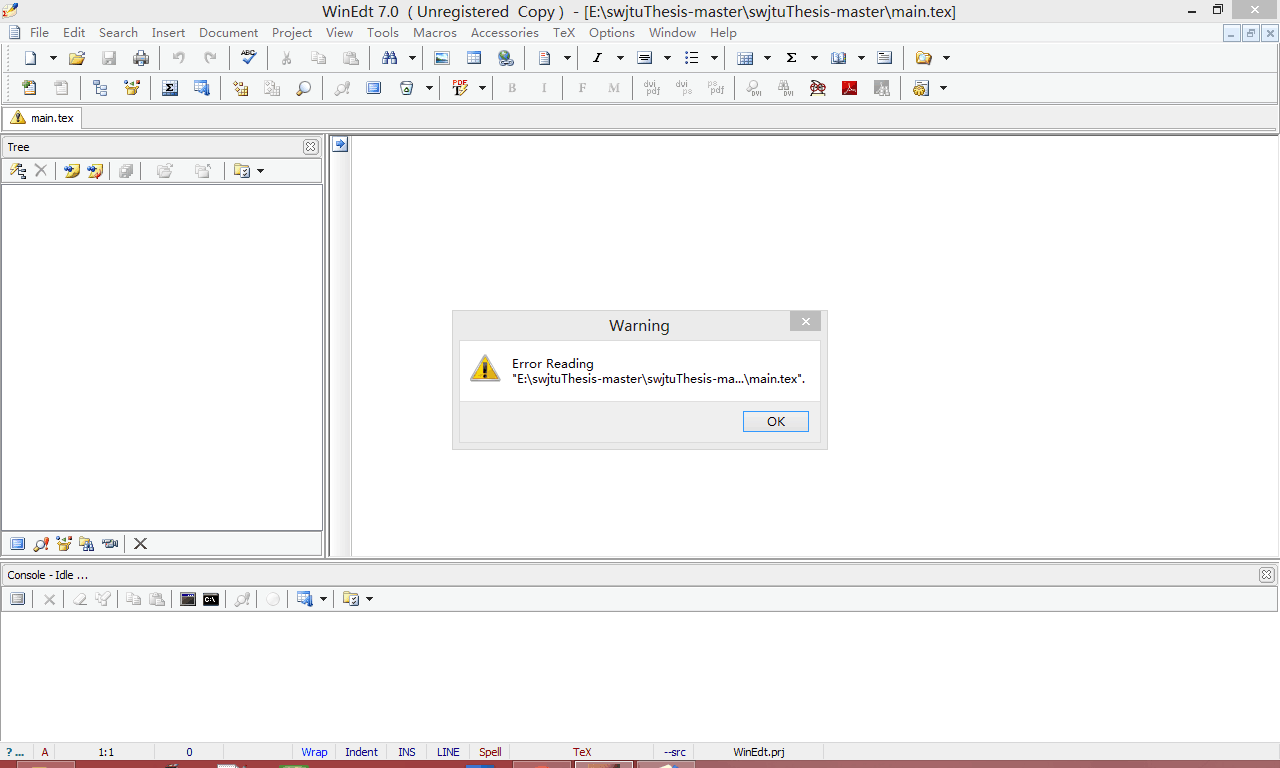
\includegraphics[width=4in]{figures/QA/Q151208_1_Yang.png}
		\caption{WinEdt打开main.tex报错}
		\label{Q151208_1_Yang}
	\end{figure}
	\item[A2:]本问题是由WinEdt编辑器内部的打开编码与模板编码不统一导致。由于swjtuThesis模板本身以及所使用的~\BibTeX{}~参考文献库均采用的是UTF-8编码。\textbf{解决办法}:在WinEdt中:点击\verb|File - Open|,然后找到main.tex文件,在右下角的编码选择处选择UTF-8,打开即可。
	\item[Q3:]
	\item[A3:]
\end{enumerate}

\subsection{排版问题}
\begin{enumerate}
	\item[Q1:]如何实现博士学位论文的页码单双页左右混合显示?
	\item[A1:]其实这是一个\textbf{单面打印}和\textbf{双面打印}功能的定义。由于swjtuThesis只采用了单一样式文件swjtuThesis.cls实现模板建立(减少模板复杂程度),针对硕士和博士的格式区分是通过引入判断字符串实现的,因为加载样式出现在判断学位种类之前,而单面打印和双面打印需要在加载样式的时候同时进行定义,因此无法通过模板自动实现此项功能。\textbf{解决办法}:如果是博士研究生,请于主文件main.tex中,修改\newline
\verb|\documentclass[oneside,openany]{swjtuThesis}|中的oneside为twoside即可手动实现双面打印功能。	
	\item[Q2:]
	\item[A2:]
\end{enumerate}

\subsection{其它问题}
\begin{enumerate}
	\item[Q1:]为什么标题页面中论文的日期是五月十三日?
	\item[A1:]纯属作者的私人原因,可以根据自己需求在info.tex文件中进行修改。
	\item[Q2:]
	\item[A2:]
\end{enumerate}

注:后续一页内容为通过\backslash\{lipsum\}生成的随机段落内容,可以通过随机内容填充版面来对照并微调版面设置

\newpage
\lipsum
%---------------------------------------------------------------------------------
%                西南交通大学研究生学位论文:第四章内容
%---------------------------------------------------------------------------------
\chapter{结束语}

尽管~\LaTeX{}~作为一款优秀且高效的科学领域排版系统,在目前国内学术圈的应用却依然相对有限,国内提供~\LaTeX{}~模板的期刊文献或者是高校均寥寥无几,在这种的环境下通过完全基于~\LaTeX{}~进行研究生学位论文的撰写的确具有一定的难度和挑战,\textbf{而这种挑战却不仅仅是学生本人在使用~\LaTeX{}~进行排版过程中遇到的困难,而更在于学生完成学位论文之后和导师的讨论和修改环节}。尽管在技术上可以通过建立GitHub项目,通过和导师协同开发进行版本控制和管理代码,以实现Word中基本的修订功能,但毕竟~\LaTeX{}~作为一门应用于页面排版的标记语言,并不是特别适合在源代码上面进行对内容的大量交互修改。作者也结合自身的经历,在次提出以下几个解决办法:

\par
\textbf{1、先在Word中撰写学位论文,修改完成后再利用swjtuThesis进行排版}。不过既然已经在Word中做好了论文撰写和编辑工作,也就并不再需要使用swjtuThesis再次进行排版,这是一种效率低下的工作方式;

\par
\textbf{2、直接把源代码发送导师阅读并修改,或者依托GitHub建立版本控制}。这样的工作方式适合和已经熟练使用,或者也打算掌握~\LaTeX{}~的导师讨论,但是无论如何基于代码的修改效率依旧不高;

\par
\textbf{3、直接把编译生成的.pdf文件打印出来和导师讨论修改}。相对来说是目前最好的解决方式,其实学位论文最重要的也只是其中的内容,科学排版的工作做得更好也只是为学位论文增色的方式之一。

\par
\textbf{在本模板的最后,但愿swjtuThesis能够帮助到更多的交大学生接触并入门~\LaTeX{}~语言,同时也能够掌握基本的~\LaTeX{}~排版方法。}

\section{免责声明}
本模板,西南交通大学研究生学位论文~\LaTeX{}~模板swjtuThesis主要依据《西南交通大学研究生学位论文撰写规范》进行编写,鉴于目前本模板仍非最终的官方版本,\textbf{作者不保证用户采用本模板撰写输出的学位论文能够完全符合学校相关要求,潜在风险和由此产生的损失由用户独自承担}。

\par
但是相对的,\textbf{作者会无条件地对在使用swjtuThesis过程中遇到技术问题的用户提供支持,也会无条件地持续对swjtuThesis进行开发和维护},直至最后取得校方认证,成为正式的西南交通大学研究生学位论文~\LaTeX{}~模板。未尽事宜,敬请谅解。


\section{修改说明}
本版本swjtuThesisV3.0是在Limin HUANG所发布的早期版本swjtuThesis\footnote{\url{https://github.com/Studio513/swjtuThesis}}以及Hao WANG所发布的V2.0修订版本\footnote{\url{https://github.com/cshaowang/swjtuThesisV2.0}}上进行进一步修订所形成的版本。这里特别声明,swjtuThesis的版权归Limin HUANG所有。如开发者Limin HUANG的初衷,虽然目前swjtuThesis作为开源项目发布,但在本模板的开发过程中,\textbf{商业转载请联系swjtuThesis开发者Limin HUANG获得授权,非商业转载请注明出处}。

% 加载论文结论
%---------------------------------------------------------------------------------
%                西南交通大学研究生学位论文:结论
%---------------------------------------------------------------------------------
\stepcounter{chapter}
\chapter*{结\qquad{}论}
\addcontentsline{toc}{chapter}{结论}
\setcounter{section}{0}

恭喜已经到达学位论文的结论部分!

\par
祝贺您在推动人类科学发展的道路上又迈进了七十亿分之一。


%---------------------------------------------------------------------------------
% 论文附录(包括致谢、参考文献、证明、工作列表)

% 加载致谢文件
%---------------------------------------------------------------------------------
%                西南交通大学研究生学位论文:致谢
%---------------------------------------------------------------------------------
\chapter*{致\qquad{}谢}
\addcontentsline{toc}{chapter}{致谢}

特别感谢Limin HUANG早期发布的swjtuThesis模板。该文档近乎全部的介绍内容也出自Limin HUANG。swjtuThesisV2.0仅依照《西南交通大学研究生学位论文撰写规范》作了轻微的修订。

\par
感谢由Hao WANG带来的swjtuThesis V2.0改进版本,该文档(V3.0)几乎所有的介绍内容均来源于Limin HUANG(V1.0)与Hao WANG(V2.0)。swjtuThesisV3.0仅依照《西南交通大学研究生学位论文撰写规范》进行了一定的优化,这些优化主要集中在版面的微调、对macOS的支持、以及对更多样的文献引用格式的支持等。

\par
希望未来能有更多的同学加入学位论文~\LaTeX{}~模板的开发和完善工作,推广~\LaTeX{}~在国内青年学生学者圈子中使用。

\vspace{25mm}
\begin{flushright}
	修订:\\
	2020年06月 \\
	2023年11月 \\
	@ 西南交大
\end{flushright}

% 加载参考文献
\clearpage
% 参考文献不分页
\interlinepenalty=10000
\phantomsection
\addcontentsline{toc}{chapter}{参考文献}
\begin{spacing}{1.2} %数字代表行距
	\setlength{\bibsep}{3pt plus1pt minus1pt}
	\bibliographystyle{ref/swjtuBST} %定义参考文献列表格式,参考国标文件GB/T 7714-2015制作
	\bibliography{ref/refEx} %加入参考文献的.bib库,可自行建立替换,refEx为示范文件
\end{spacing}

% 加载附录文件和个人工作列表
%---------------------------------------------------------------------------------
%                西南交通大学研究生学位论文:附录A
%---------------------------------------------------------------------------------
% 附录部分的可操作性很强,可以是部分测试数据、数学证明或者是个人简介,请根据需求修改
\chapter*{附录~A}							% 附录环节属于无编号章节
\addcontentsline{toc}{chapter}{附录~A}	% 定义字符串,把无编号章节加入目录中(如附录A)						% 非必要章节,主要用以放置测试数据、数学证明或者个人简介
%---------------------------------------------------------------------------------
%                西南交通大学研究生学位论文:所取得的科研成果
%---------------------------------------------------------------------------------
\chapter*{攻读\cDegree{}学位期间取得的研究成果}
\addcontentsline{toc}{chapter}{攻读\cDegree{}学位期间取得的研究成果}



一、攻读\cDegree{}学位期间发表的论文及科研成果
\begin{publist}
	\item 论文在这里.
	
	\item ..
	
\end{publist}

二、参与科研项目/科研获奖等
\begin{publist}
	\item 参与项目在这里.
	
	\item ..
\end{publist}					% 攻读硕(博)士论文攻读期间取得的科研成果,论文、专利等

\end{document}
